%
% stueckweise.tex
%
% (c) 2019 Prof Dr Andreas Müller, Hochschule Rapperswil
%
\section{Stückweise konstante Funktionen%
\label{section:stueckweise}}
\rhead{Stückweise konstante Funktionen}
Eine Funktion $f\colon[a,b]\to\mathbb R$ heisst {\em stückweise konstant},
\index{stückweise konstant}
wenn es eine Unterteilung des Intervalls $[a,b]$ durch Punkte
\index{Unterteilung}%
$x_k\in\mathbb R$ mit $0\le k\le n$ gibt, also
\[
a=x_0 < x_1 < \dots < x_k < \dots < x_{n-1} < x_n = b,
\]
so dass die Funktion $f$ in jedem Teilintervall $[x_k,x_{k+1})$
konstant ist.
Es gibt also eine Menge von Zahlen $f_k$ derart, dass
\begin{equation}
f(x)
=
f_k
\qquad\text{falls}\qquad
x_k \le x < x_{k+1}.
\label{buch:stückweisef}
\end{equation}
Stückweise konstante Funktionen sind natürlich nicht überall stetig,
vielmehr ist jeder der Punkte $x_k$ eine potentielle Unstetigkeitsstelle.
Es gilt nämlich
\begin{equation*}
\begin{aligned}
\lim_{x\to x_k-} f(x)
&=
f_{k-1}&\forall k\text{ mit }&1\le k \le n,
\\
\lim_{x\to x_k+} f(x)
&=
f_k&\forall k\text{ mit }&0\le k \le n-1.
\end{aligned}
\end{equation*}
Wenn also $f_k\ne f_{k-1}$, dann ist $x_k$ eine Unstetigkeitsstelle.
$f(x)$ ist immer noch rechtsseitig stetig, aber der linksseitige
Grenzwert ist verschieden, die Funktion hat einen Sprung an der
Stelle $x_k$.

\subsection{Indikatorfunktion}
\begin{figure}
\centering
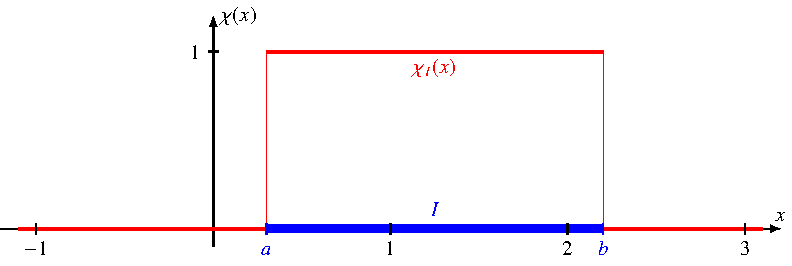
\includegraphics{chapters/3-haar/images/chi.pdf}
\caption{Indikatorfunktion oder charakteristische Funktion $\chi_I(t)$
des Intervalls $I=[a,b]\subset \mathbb R$ (vgl. auch \eqref{formel:chi}).
\label{haar:figure:chi}}
\end{figure}
Mit Hilfe der Indikatorfunktion %oder charakteristischen Funktion
eines Intervalls lässt sich eine stückweise konstante Funktion etwas
eleganter schreiben.
Wir definieren  die
{\em Indikatorfunktion}
\index{Indikatorfunktion}%
oder
{\em charakteristische Funktion}
\index{charakteristische Funktion}
des Intervalls $I$ als
\begin{equation}
\chi_{I}(x) = \begin{cases}
1&\qquad x\in I\\
0&\qquad x\not\in I
\end{cases}
\label{formel:chi}
\end{equation}
(siehe auch Abbildung~\ref{haar:figure:chi}).
Damit kann man die stückweise konstante Funktion $f(x)$ aus
\eqref{buch:stückweisef}
als Linearkombination
\[
f(x)
=
\sum_{k=0}^{n-1} f_k\chi_{[x_k,x_{k+1})}(x)
\]
von Indikatorfunktionen schreiben.

\subsection{Approximation stetiger Funktionen}
\begin{figure}
\centering
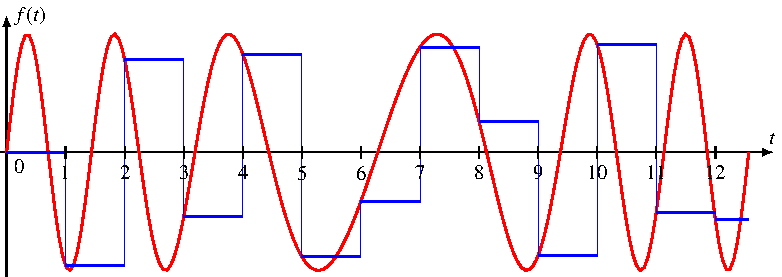
\includegraphics{chapters/3-haar/images/stueckweise1.pdf}
\caption{Stückweise konstante Approximation einer Funktion $f(t)$ mit
Mit Hilfe einer Unterteilung der $t$-Achse in Intervalle der Länge $1$.
Die Approximation ist zu grob, wesentliche Eigenschaften der
Funktion können nicht wiedergegeben werden.
\label{haar:approximation1:image}}
\end{figure}
\begin{figure}
\centering
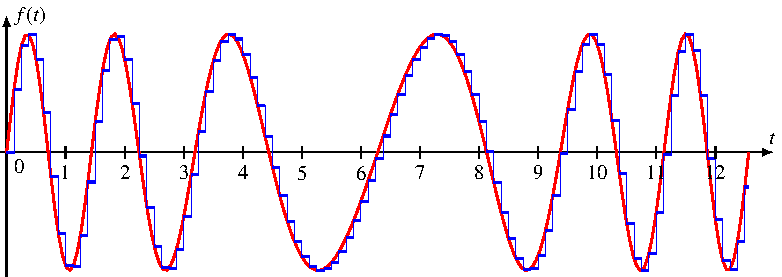
\includegraphics{chapters/3-haar/images/stueckweise8.pdf}
\caption{Stückweise konstante Approximation einer Funktion $f(t)$ mit
Mit Hilfe einer Unterteilung der $t$-Achse in Intervalle der Länge $\frac18$.
Die wesentlichen Eigenschaften der Funktion $f(t)$ sind nachvollziehbar,
aber es sind immer noch beträchtliche Unterschiede erkennbar.
\label{haar:approximation8:image}}
\end{figure}
\begin{figure}
\centering
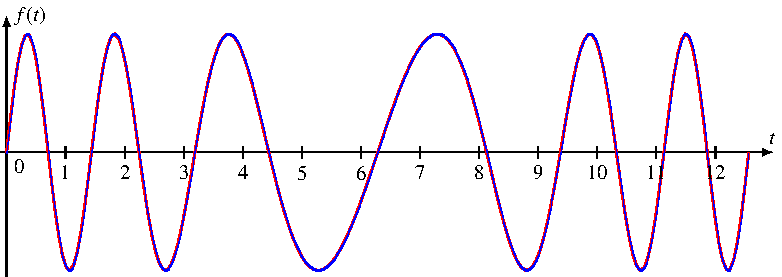
\includegraphics{chapters/3-haar/images/stueckweise64.pdf}
\caption{Stückweise konstante Approximation einer Funktion $f(t)$ mit
Mit Hilfe einer Unterteilung der $t$-Achse in Intervalle der Länge $\frac1{64}$.
Die Approximation ist so gut, dass man kaum mehr einen Unterschied
zwischen Approximation und approximierter Funktion erkennen kann.
\label{haar:approximation64:image}}
\end{figure}
Stückweise konstante Funktionen sind zwar nicht stetig, aber sie können
stetige Funktionen beliebig genau approximieren.
Dazu ist aber auch nötig, die Punkte $x_k$ genügen nahe beeinander zu
haben.
Als Mass dafür definieren wir das {\em Korn} einer Unterteilung:
\index{Korn}%

\begin{definition}
Die grösste Länge eines Teilintervalls einer Unterteilung $U$
\[
\delta(U)
=
\delta(\{x_0,\dots,x_n\})
=
\max_{0\le k < n} (x_{k+1}-x_{k})
\]
heisst das {\em Korn} der Unterteilung.
\end{definition}

Es wird also behauptet, dass eine stetige Funktion durch eine stückweise
konstante Funktion beliebig genau approximiert werden kann, wenn das
Korn der Unterteilung klein genug gemacht wird.
Um dies genauer auszudrücken, sei jetzt $\varepsilon >0$ gegeben.
Da die Funktion $f(x)$ stetig ist, gibt es eine Zahl $\delta>0$ derart,
dass
\[
|f(x) - f(y)| < \varepsilon\qquad\forall x,y\in [a,b]\quad\text{mit}\quad
|x-y|<\delta.
\]
Man wählt nun eine Unterteilung des Intervalls mit Korn
$\delta(\{x_0,\dots,x_n\}) < \delta$ und setzt
\[
g_k = f(x_k),\quad 0\le k < n.
\]
Die Zahlen $g_k$ definieren eine stückweise konstante Funktion $g$, die 
die Funktion $f$ mit maximalem Fehler $\varepsilon$ approximiert:
\[
|f(x)-g(x)|
=
|f(x) - f(x_k) + f(x_k) - g(x_k)|
\le
|f(x) - f(x_k)| + |f(x_k) - g(x_k)|
<
\varepsilon + 0
\]
für $x\in [x_k,x_{k+1})$.

\subsection{Obere und untere Approximation}
Sei $f$ ein stetige Funktion und $\{x_0,\dots,x_n\}$ eine Unterteilung
des Intervalls $[a,b]$.
Dann kann man sofort zwei weitere stückweise konstanten Approximationen 
konstruieren, die {\em obere Approximation}
\begin{align*}
&\hspace{3cm}&
\overline{f}(x)
&= 
\sup_{x\in[x_k,x_{k+1})} f(x)
&\text{falls }&x\in[x_k,x_{k+1}]
&\hspace{3cm}&
\intertext{und die {\em untere Approximation}}
&\hspace{3cm}&
\underline{f}(x)
&= 
\inf_{x\in[x_k,x_{k+1})} f(x)
&\text{falls }&x\in[x_k,x_{k+1}].
&\hspace{3cm}&
\end{align*}
Die Funktion $\overline{f}$ ist also immer mindestens so gross wie $f$
und $\underline{f}$ ist immer höchstens so gross wie $f$.
Es gilt also
\[
\underline{f}(x) \le f(x) \le \overline{f}(x)
\]
für $x\in[a,b]$.
Ausserdem gilt für die weiter oben konstruierte Approximation $g(x)$ der
Funktion $f(x)$ die Ungleichung
\[
\underline{f}(x) \le g(x) \le \overline{f}(x)
\]
für $x\in[a,b]$.

Man kann die obere und untere Approximation kann auch als Linearkombination
\begin{align*}
\overline{f}
&=
\sum_{k\in\mathbb Z} \sup_{x\in[x_k,x_{k+1})}f(x)\cdot \chi_{[x_k,x_{k+1})},
\\
\underline{f}
&=
\sum_{k\in\mathbb Z} \inf{x\in[x_k,x_{k+1})}f(x)\cdot \chi_{[x_k,x_{k+1})}
\end{align*}
von Indikatorfunktionen schreiben.

\subsection{Vektorraum der stückweise stetigen Funktionen}
Die stetigen Funktionen auf einem Intervall bilden einen Vektorraum: eine
Summe von stetigen Funktionen ist wieder eine stetige Funktionen.
Intuitiv ist auch klar, dass ein Summe stückweise konstanter Funktionen
wieder stückweise konstant ist.
Es ist aber auch klar, dass die Summe zweier Funktionen, die verschiedene
Unterteilungen verwenden, im allgemeinen mit keiner der Unterteilungen
stückweise konstant ist.
Seien $U_f=\{x_0^{(f)},\dots,x_n^{(f)}\}$ und
$U_g=\{x_0^{(g)},\dots,x_m^{(g)}\}$ die Unterteilung, bezüglich der 
die Funktionen $f$ und $g$ stückweise konstant sind.
Dann ist die Vereinigungsmenge
\[
U= \{x_0,\dots,x_N\} = U_f\cup U_g
\]
eine Unterteilung von $[a,b]$.
Da alle Teilpunkte von $U_f$ in $U$ sind, ist $f$ auch eine stückweise
konstante Funktion bezüglich der Unterteilung $U$. 
Ebenso ist $g$ eine stückweise konstante Funktion bezüglich $U$.
Da $U$ eine gemeinsame Unterteilung für $f$ und $g$ ist, kann man
die Summe $h=f+g$ als stückweise konstante Funktion mit
\[
h_k
=
(f+g)(x_k)
= 
f(x_k) + f(x_k)
\qquad\text{mit}\quad
0\le k\le N
\]
betrachten.
Die Vereinigung der Unterteilungen stellt also sicher, dass sich
zu zwei beliebigen stückweise konstanten Funktionen immer eine
gemeinsame Unterteilung finden lässt, die klar macht, dass $f+g$
wieder eine stückweise konstante Funktion ist.

Die vom Funktionenraum geerbte Vektorraumstruktur verlangt zwar etwas
mehr Sorgfalt bei der Verifikation, darf aber als gegeben angesehen
werden.

\subsection{Integration stückweise konstanter Funktionen}
Das Integral einer stückweise konstanten Funktion ist besonders einfach 
zu berechnen, nämlich
\[
\int_{\mathbb R} f(x)\,dx = \sum_{k=0}^{n-1} f_k\cdot (x_{k+1}-x_k).
\]
Dies ist im wesentlichen die Definition des {\em Riemann-Integrals}.
\index{Riemann-Integral}%
Genauer wird das Riemann-Integral einer stetigen Funktion jeweils
konstruiert mit Hilfe von genügend feinen Unterteilungen und den
Approximationen $\overline{f}$ und $\underline{f}$.
Dazu bildet man die Integrale
\begin{align*}
\int_a^b \underline{f}(x)\,dx
=
\sum_{k=0}^{n-1} \underline{f}_{k}\,(x_{k+1}-x_k)
\le
\sum_{k=0}^{n-1} \overline{f}_{k}\,(x_{k+1}-x_k)
=
\int_a^b \overline{f}(x)\,dx.
\end{align*}
Verfeinerung des Korns der verwendeten Unterteilung bringt für eine
stetige Funktion die beiden Schranken näher zusammen.
Das Integral der stetigen Funktion $f(x)$ ist dann der Grenzwert
dieser beiden Schranken:
\[
\lim_{\delta\to 0}
\int_a^b \underline{f}(x)\,dx
=
\int_a^b f(x)\,dx
=
\lim_{\delta\to 0}
\int_a^b \overline{f}(x)\,dx,
\]
wobei für den Grenzwert Unterteilungen verwendet werden sollen, deren
Korn $\delta$ gegen $0$ geht.
Das Riemann-Integral verträgt sich daher gut mit den arithmetischen
Operationen: es ist eine lineare Abbildung.
Es verträgt sich aber auch mit dem Begriff der Approximation von
stetigen Funktionen: nahe beeinanderliegende Funktionen haben nahe
beeinanderliegende Integrale.

\subsection{Skalarprodukt}
Die stückweise konstanten Funktionen bilden aber auch einen Vektorraum
mit Skalarprodukt.
Das Skalarprodukt ist wie in Kapitel~\ref{chapter:fourier} definiert durch
\[
\langle f,g\rangle
=
\int_a^b
f(x) g(x)\,dx.
\]
Ist $U$ eine gemeinsame Unterteilung für die stückweise konstanten
Funktionen $f$ und $g$, dann ist das Skalarprodukt
\[
\langle f,g\rangle
=
\sum_{k=0}^{n-1} f(x_k) g(x_k) \cdot |x_{k+1}-x_{k\mathstrut}|.
\]
Das Skalarprodukt hat also bis auf die Faktoren $|x_{k+1}-x_{k\mathstrut}|$
die gleiche Form wie das Skalarprodukt in einem endlichdimensionalen
Vektorraum.
Daraus kann zum Beispiel geschlossen werden, dass für dieses Skalarprodukt
die Cauchy-Schwarz-Ungleichung gilt und dass es positiv definit ist.

Der Vektorraum der stückweise konstanten Funktionen kann nicht vollständig
sein.
Jede stetige Funktion ist ein Grenzwert von stückweise konstanten
Funktionen.
Selbstverständlich kann man auf analoge Art auch einen komplexen
Vektorraum mit hermitschem Skalarprodukt konstruieren.
Weil er nicht vollständig ist, kann er kein Hilbertraum sein.
Um ihn besser zu verstehen wäre es schön, wenn man eine Hilbert-Basis
angeben könnte, also eine Folge von orthonormierten Funktionen, mit
denen man jede Funktion approximieren kann.
Die vielen möglichen Teilpunkte des Intervalls sind dafür aber eher 
hinderlich.

